%% Progetto di linguaggi di programmazione - Gianluca Grilletti e Giovanni Barbarino
%% Semantica Fully Abstract per PCF


\documentclass{beamer}

\usepackage[utf8]{inputenc}
\usepackage{default}
\usepackage{amssymb}
\usepackage{stmaryrd}
\usepackage{graphicx}
\usepackage{caption}
%\usepackage{subcaption}
\usepackage{tikz}
\usetikzlibrary{arrows,automata}
\newcommand{\eqobs}{\stackrel{\text{obs}}{=}}
\newcommand{\limp}{\mathbin{{-}\mkern-3.5mu{\circ}}}
\newcommand{\tnode}[4]{\node (#1_u) at (#2,#3+0.1) [minimum size=2pt, opacity=0] {#4};
		       \node (#1_d) at (#2,#3-0.1) [minimum size=2pt, opacity=0] {#4};
		       \node (#1) at (#2,#3) [minimum size=2pt] {#4};}


% immagini
\graphicspath{{immagini/}}




\usetheme{Darmstadt}

\title{Un modello fully abstract del PCF}
% \subtitle{Vuoi fare un gioco con me?}
\author{Grilletti Gianluca \and Barbarino Giovanni}
\institute[Unipi]{Università di Pisa}


\begin{document}

\small




%titolo
\begin{frame}
	%\frametitle{Il linguaggio PCF}
	\maketitle
	
\end{frame}



% prova di implicazione
\begin{frame}
\frametitle{Il gioco $A\Rightarrow B$}

\only<2->{
	\[
	A \Rightarrow B \quad \equiv \quad !A \limp B
	\]
}

\onslide<3->{
\begin{itemize}
 \item $Gun=A$ con $P_A=\{
 \only<3-5>{\textcolor{red}{\epsilon}} \only<1-2,6->{\epsilon},
 \;  \only<6,8>{\textcolor{red}{\underline{pull}}} \only<1-5,7,9->{\underline{pull}}, 
 \; \only<7>{\textcolor{red}{\underline{pull}\:click}} \only<1-6,8->{\underline{pull}\:click}, 
 \; \only<9->{\textcolor{red}{\underline{pull}\:bang}} \only<1-8>{\underline{pull}\:bang} 
 \}$
 \item $Life=B$ con $P_B=\{
 \only<3-4>{\textcolor{red}{\epsilon}} \only<1-2,5->{\epsilon},
 \;  \only<5-9>{\textcolor{red}{*_O}} \only<1-4,10->{*_O}, 
 \; *_O\checkmark_P,
 \; *_O1_P,
 \; \only<10->{\textcolor{red}{*_O2_P}} \only<1-9>{*_O2_P},
 \; *_O3_P,
 \; \dots \}$
 \item<4-> Strategia \textit{Roulette Russa}:
 
 $\only<6>{\textcolor{red}{f(*_O)=\underline{pull}_1}} \only<4-5,7->{f(*_O)=\underline{pull}_1}$, 
 $\quad \only<8>{\textcolor{red}{f(click_n)=\underline{pull}_{n+1}}} \only<4-7,9->{f(click_n)=\underline{pull}_{n+1}} \forall n$,  
 $\quad \only<10>{\textcolor{red}{f(bang_n)=n_P}} \only<4-9>{f(bang_n)=n_P}$
\end{itemize}
}



\only<2->{ 
	\begin{tikzpicture}
	 \node (inv) at (0,0) [minimum size=2pt] {};
	 \node (inv2) at (11,-4) [minimum size=2pt] {};
	 \foreach \x in {0,3,6} { 
	  \draw [fill=blue, opacity=.5] (\x+2,-3) rectangle (\x,-1);
	 % \node (A) at (\x+1,-2) [minimum size=2pt, scale=2] {A};
	  \node (P) at (\x+0.3,-1.3) [minimum size=2pt, scale=1.5] {P};
 	  \node (O) at (\x+0.3,-2.7) [minimum size=2pt, scale=1.5] {O};
	  }
	  \node (A) at (7,-2) [minimum size=2pt, scale=2] {A$_1$};
	  \node (A) at (4,-2) [minimum size=2pt, scale=2] {A$_2$};
	  \node (A) at (1,-2) [minimum size=2pt, scale=2] {A$_3$};
	 \draw [fill=red, opacity=.5] (11,-3) rectangle (9,-1);
	 \node (B) at (10,-2) [minimum size=2pt, scale=2] {B};
	 \node (P) at (9.3,-2.7) [minimum size=2pt, scale=1.5] {P};
 	 \node (O) at (9.3,-1.3) [minimum size=2pt, scale=1.5] {O};
	 
	 \only<5->{\node (st1) at (10,-0.5) [minimum size=2pt, scale=1.5] {$*_O$};}
 	 \only<6->{\node (st2) at (7,-0.5) [minimum size=2pt, scale=1.5] {$\underline{pull}_1$};}
	 \only<7->{\node (ri2) at (7,-3.5) [minimum size=2pt, scale=1.5] {$click_1$};}
 	 \only<8->{\node (st3) at (4,-0.5) [minimum size=2pt, scale=1.5] {$\underline{pull}_2$};}
	 \only<9->{\node (ri3) at (4,-3.5) [minimum size=2pt, scale=1.5] {$bang_2$};}
 	 \only<10->{\node (ri1) at (10,-3.5) [minimum size=2pt, scale=1.5] {$2_P$};}
 	 
	  \only<6->{\draw[->] [out=250,in=280] (st1) to (st2);}
	  \only<7->{\draw[->] [out=250,in=30] (st2) to (ri2);}
	  \only<8->{\draw[->] [out=80,in=280] (ri2) to (st3);}
	  \only<9->{\draw[->] [out=250,in=110] (st3) to (ri3);}
	  \only<10->{\draw[->] [out=30,in=150] (ri3) to (ri1);}
	  \end{tikzpicture}

	}
	
	
\end{frame}




\end{document}
